\documentclass[final]{beamer}
\usepackage[scale=1.24]{beamerposter}
\usepackage{graphicx,booktabs} 
\usepackage{helvet}

\usetheme{confposter}
\setbeamercolor{block title}{fg=Maroon,bg=white}
\setbeamercolor{block body}{fg=black,bg=white}
\setbeamercolor{block alerted title}{fg=white,bg=Maroon!70}
\setbeamercolor{block alerted body}{fg=black,bg=Maroon!10} 

\newlength{\sepwid}
\newlength{\onecolwid}
\newlength{\twocolwid}
\newlength{\threecolwid}
\setlength{\paperwidth}{48in}
\setlength{\paperheight}{36in}
\setlength{\sepwid}{0.024\paperwidth}
\setlength{\onecolwid}{0.22\paperwidth}
\setlength{\twocolwid}{0.464\paperwidth}
\setlength{\threecolwid}{0.708\paperwidth}
\setlength{\topmargin}{-0.5in}

\title{Fido: A Universal Robot Control System using\\Reinforcement Learning with Limited Feedback}
\author{Joshua Gruenstein \and Michael Truell}
\institute{Horace Mann School}

\begin{document}

\addtobeamertemplate{block end}{}{\vspace*{2ex}}
\addtobeamertemplate{block alerted end}{}{\vspace*{2ex}}
\setlength{\belowcaptionskip}{2ex}
\setlength\belowdisplayshortskip{2ex}

\begin{frame}[t]
\begin{columns}[t]

\begin{column}{\sepwid}\end{column}

\begin{column}{\onecolwid}


	\begin{alertblock}{Control System Objectives}
		Fido was created to fulfill the following two goals:
		\begin{itemize}
			\item \textbf{Trainability}: Allow both human and autonomous training rather than reprogramming
			\item \textbf{Universality}: Run on any robot, even without prior knowledge of the host
		\end{itemize}
		These goals were achieved through the training of artificial neural networks with a wire-fitted moving least squares interpolator following the Q-learning reinforcement algorithm and an action selection policy that utilizes a Boltzmann distribution of probability.
	\end{alertblock}


\begin{figure}
	\centering
	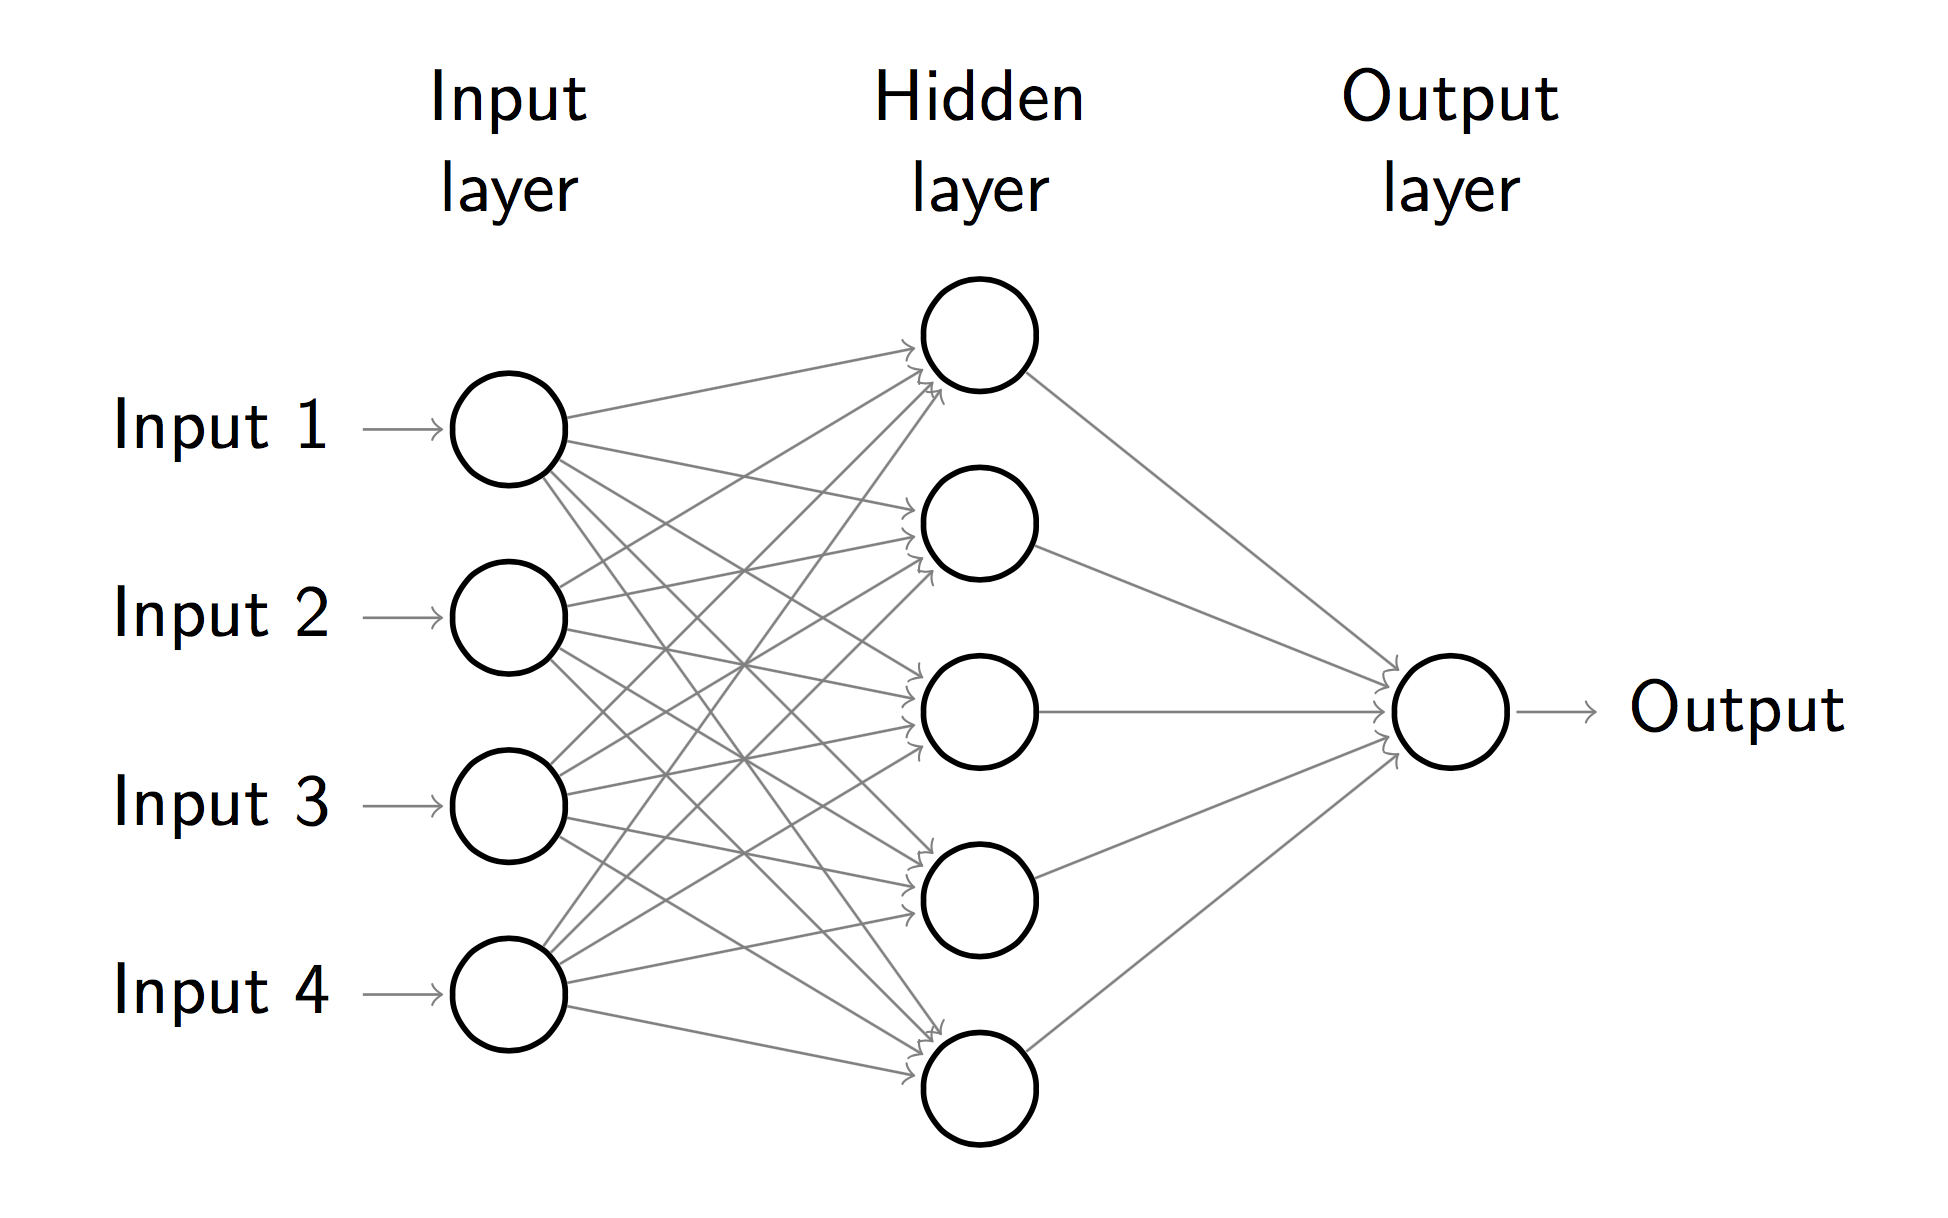
\includegraphics[width=\linewidth]{Figures/FeedForwardRendered}
	\caption{Single Output Feed-forward Neural Network}
	\label{fig:feedforward}
\end{figure}

%----------------------------------------------------------------------------------------

\end{column}

\begin{column}{\sepwid}\end{column} 

\begin{column}{\twocolwid}

	\begin{block}{Learning Algorithm}

		The following materials were required to complete the research:

		\begin{itemize}
		\item Curabitur pellentesque dignissim
		\item Eu facilisis est tempus quis
		\item Duis porta consequat lorem
		\item Eu facilisis est tempus quis
		\end{itemize}

		The materials were prepared according to the steps outlined below:

		\begin{enumerate}
		\item Curabitur pellentesque dignissim
		\item Eu facilisis est tempus quis
		\item Duis porta consequat lorem
		\item Curabitur pellentesque dignissim
		\end{enumerate}

	\end{block}

\begin{alertblock}{Important Result}

Lorem ipsum dolor \textbf{sit amet}, consectetur adipiscing elit. Sed commodo molestie porta. Sed ultrices scelerisque sapien ac commodo. Donec ut volutpat elit.

\end{alertblock} 

%----------------------------------------------------------------------------------------

\begin{columns}[t,totalwidth=\twocolwid]

\begin{column}{\onecolwid}\begin{block}{Simulation}

	Hello.

\end{block}\end{column}

\begin{column}{\onecolwid}\begin{block}{Hardware Implementation}
	
	Hi.

\end{block}\end{column} 

\end{columns} 

\end{column}

\begin{column}{\sepwid}\end{column}

\begin{column}{\onecolwid}

	\begin{block}{Future Development}
		Nunc tempus venenatis facilisis. \textbf{Curabitur suscipit} consequat eros non porttitor. Sed a massa dolor, id ornare enim. Fusce quis massa dictum tortor \textbf{tincidunt mattis}. Donec quam est, lobortis quis pretium at, laoreet scelerisque lacus. Nam quis odio enim, in molestie libero. Vivamus cursus mi at \textit{nulla elementum sollicitudin}.
	\end{block}


	\begin{block}{References}
		\nocite{*}
		\small{\bibliographystyle{IEEEtran}\bibliography{Poster}\vspace{0.75in}}
	\end{block}

	\setbeamercolor{block title}{fg=dblue,bg=white}
	\begin{block}{Acknowledgements}
		\small{\rmfamily{Thank you to Dr. Jeff Weitz from Horace Mann School, who gave us guidance in the art of scientific research.}}
	\end{block}


\end{column}

\end{columns}
\end{frame}
\end{document}

%%%%%%%%%%%%%%%%%%%%%%%%%%%%%%%%%%%%%%%%%
% Adapted from "Jacobs Landscape Poster" 
% (https://teamwork.jacobs-university.de:8443/confluence/display/CoPandBiG/LaTeX+Poster)
% License: CC BY-NC-SA 3.0 (http://creativecommons.org/licenses/by-nc-sa/3.0/)
%%%%%%%%%%%%%%%%%%%%%%%%%%%%%%%%%%%%%%%%%
